\documentclass[conference]{IEEEtran}
\IEEEoverridecommandlockouts
\usepackage{cite}
\usepackage{amsmath,amssymb,amsfonts}
\usepackage{graphicx}
\usepackage{booktabs}
\usepackage{multirow}
\usepackage{xcolor}
\usepackage{url}
\graphicspath{{figures/}}

\begin{document}

\title{ARGUS: Measuring Adversarial Degradation and Recovery of Temporal Graph Neural Networks for Cross-Bank Anti-Money Laundering}

\author{
\IEEEauthorblockN{Y. Charan Sai, B. Ram Charan, C. Ganesh Kumar}
\IEEEauthorblockA{Department of Artificial Intelligence and Data Science\\
Chaitanya Bharathi Institute of Technology, Hyderabad, India}
\and
\IEEEauthorblockN{V. Vasuki Rohini Devi}
\IEEEauthorblockA{Department of Artificial Intelligence and Data Science\\
Chaitanya Bharathi Institute of Technology, Hyderabad, India}
% Add e-mail addresses as \\ name@domain lines inside each \IEEEauthorblockA if the venue requires them.
}

\maketitle

\begin{abstract}
Proceeds of cyber fraud are laundered within minutes through chains of mule accounts spread across banks, so no single bank observes the laundering ring. Graph neural networks (GNNs) detect such rings well on fixed benchmarks, but they are rarely evaluated against launderers who adapt after detection. We present ARGUS, which pairs a heterogeneous, time-respecting edge-level GNN with a multi-bank digital twin in which laundering rings with complete ground truth are injected into real background traffic and mutated by an attacker. On the IBM AML HI-Small benchmark (5.08\,M transactions, chronological test split), the GNN reaches a PR-AUC of 0.726 and an F1 of 0.729, against 0.296 and 0.367 for LightGBM on identical features, and fully recovers 60.4\% of laundering rings against 4.2\%. Restricting neighbour sampling to the past of each scored transaction changes PR-AUC by less than 0.01. On the twin we measure, for six attack tactics and for an adaptive multi-round attacker, the degradation $D$ an attack causes and the recovery $R$ retraining achieves. The graph model largely neutralises structuring ($D$=0.038 vs.\ 0.439 for LightGBM) and feature mimicry ($D$=0.102 vs.\ 0.307), whereas relation camouflage --- mules padding their neighbourhoods with legitimate counterparties --- costs both models 0.44--0.48 F1 and is only partly recovered. An investigation agent reconstructs detected rings with a Jaccard similarity of 0.90 and drafts suspicious transaction reports whose language-model narrative is checked number by number against computed facts.
\end{abstract}

\begin{IEEEkeywords}
anti-money laundering, graph neural networks, temporal graphs, adversarial robustness, digital twin, mule accounts
\end{IEEEkeywords}

\section{Introduction}
When a fraud victim transfers money, the funds are split and forwarded through mule accounts at several banks and withdrawn as cash within minutes. Each bank sees a single hop that looks ordinary in isolation; the laundering pattern exists only in the network. Rule-based monitoring, which flags individual transactions by fixed thresholds, is evaded by staying below the thresholds and produces many false alarms. Graph learning addresses the representation problem: heterogeneous and temporal GNNs outperform flat models for anti-money laundering (AML) \cite{johannessen2025finding, digennaro2024amatriciana, alarab2023graph}, and regulators are deploying AI-based mule detection \cite{rbih2024mulehunter}.

Detection on a static benchmark, however, is the easy part. Launderers observe which accounts are frozen and change tactics: they structure transfers, slow the ring down, imitate normal payment formats, or surround mules with ordinary-looking activity. Prior work evaluates adaptive attackers in promotion fraud \cite{prasetya2025multi} and camouflage in review fraud \cite{dou2020enhancing}, but no work we are aware of measures, for bank AML, how much accuracy an adaptive launderer removes from a graph detector and how much retraining wins back.

\textbf{Contributions.} (1) A leakage-safe pipeline on IBM AML HI-Small \cite{altman2023realistic} with chronological splits, past-only features, validation-chosen thresholds and time-respecting neighbour sampling. (2) A heterogeneous edge-level GNN over accounts, owning entities and banks that more than doubles the PR-AUC of a gradient-boosting model on the same features. (3) A multi-bank digital twin with six attack operators and a protocol that reports degradation $D$ and recovery $R$, including under an adaptive multi-round attacker. (4) An investigation agent with a grounding check for language-model reports.

\section{Related Work}
\textbf{Graph representations for AML.} Johannessen and Jullum \cite{johannessen2025finding} introduce heterogeneous GNNs over customers, accounts and banks on private single-bank data. Amatriciana \cite{digennaro2024amatriciana} combines GraphSAGE with an LSTM on IBM data and reduces false positives by 55\%; Alarab and Prakoonwit \cite{alarab2023graph} find that temporal GCNs beat static ones on Bitcoin. Egressy et al. \cite{egressy2024provably} add multigraph-specific message passing for IBM AML. Bellei et al. \cite{bellei2024shape} argue for subgraph-level detection with Elliptic2.

\textbf{Data.} Labelled laundering data is scarce, so simulators with injected, labelled patterns are standard: AMLSim \cite{weber2018scalable}, agent-based models with GANs \cite{granados2024gan}, and the IBM AML generator \cite{altman2023realistic}.

\textbf{Robustness and constraints.} Prasetya et al. \cite{prasetya2025multi} show that fraud detectors collapse below 0.56 F1 when fraudsters adapt over rounds. CARE-GNN \cite{dou2020enhancing} names feature and relation camouflage and filters neighbours accordingly. PC-GNN \cite{liu2021pick} and LaundroGraph \cite{cardoso2022laundrograph} address imbalance and label scarcity. None of these measures degradation and recovery for bank AML in a controlled multi-bank setting; ARGUS combines these threads in one protocol.

\section{Data and Leakage-Safe Protocol}
HI-Small contains 5,078,345 transactions among 515,088 accounts at 30,470 banks, of which 0.102\% are laundering; an ownership file links 518,581 accounts to 166,207 entities. Transactions are sorted by time and split 60/20/20 into train (3.05\,M, 0.075\% positive), validation (1.02\,M, 0.107\%) and test (1.02\,M, 0.177\%) periods. All 17 per-transaction features use only the transaction and earlier activity: amount, currency hop, cross-bank flag, time of day, payment format, 24-hour fan-out and fan-in of the sender and receiver, pass-through indicators, prior activity counts, time since the sender's previous transfer and amount relative to the sender's history. The decision threshold maximises F1 on validation and is fixed for test. We report PR-AUC and laundering-class precision, recall and F1, never accuracy, and ring recall: the share of known laundering attempts with all transfers flagged.

\section{Detector}
\textbf{Graph.} Accounts, entities and banks are nodes. Each transaction is an edge carrying a 40-dimensional feature vector and a timestamp; reverse edges let messages flow against the money. Static ownership and bank-membership edges connect accounts to their owners and banks; 67\% of laundering accounts belong to entities owning several accounts.

\textbf{Model.} Each of two layers applies a relation-specific convolution and sums per node type, with layer normalisation, dropout and a residual connection. Transaction relations use edge-aware GINE \cite{hu2020strategies}; other relations use GraphSAGE. A transaction $e=(u,v)$ is scored as $\hat{y}_e=\sigma(\mathrm{MLP}([\mathbf{h}_u \Vert \mathbf{h}_v \Vert \phi(\mathbf{x}_e)]))$ and trained with weighted binary cross-entropy ($w_+=5$), hidden size 64, AdamW and early stopping on validation PR-AUC, using PyTorch Geometric \cite{fey2019fast}.

\textbf{Time-respecting sampling.} Mini-batches are built by neighbour sampling. A naive sampler on the full test-period graph lets the neighbourhood of a scored transaction include \emph{later} transactions --- no labels leak, but the model sees information unavailable at decision time. We restrict sampling to $\mathcal{N}_{\le t}(v)=\{u:(u,v,t')\in E,\ t'\le t\}$ with per-seed subgraphs; an automated test asserts that no sampled transaction is later than its seed.

\textbf{Baselines.} Five fixed-threshold rules fitted on the training period (amount, fan-out, fan-in, pass-through, currency hop), and LightGBM \cite{ke2017lightgbm} on the same 17 features. Weighting the positive class by the class ratio ($\approx$1300) saturated LightGBM's scores and cut PR-AUC from 0.296 to 0.007; the unweighted model is reported.

\section{Adversarial Evaluation}
\textbf{Digital twin.} To measure attacks we need laundering whose structure is fully known. The twin keeps the normal traffic among the eight busiest HI-Small banks (99,289 transactions, 44\% cross-bank) and removes IBM's own laundering. It injects 400 rings (3,348 laundering transactions) uniformly in time as chains, fan-outs, scatter--gathers and cycles; each hop crosses banks, takes minutes and loses a small fee. Mules are recruited dormant accounts or freshly opened ones, often sharing an owner. Each ring stays within the period in which it starts, so attacks can target test rings only.

\textbf{Attack operators.} \emph{separate\_owners} gives fresh mules distinct owners; \emph{add\_hops} routes every transfer through an extra mule at another bank; \emph{split} structures each transfer into 2--4 smaller ones; \emph{delay} stretches the ring from minutes to hours; \emph{mimic} draws payment formats and currencies from normal traffic (feature camouflage); \emph{camouflage} makes each mule transact normally with 3--8 legitimate accounts (relation camouflage).

\textbf{Protocol.} A detector trained on the clean twin is evaluated on test rings mutated by an operator, giving $D=F_1^{\text{before}}-F_1^{\text{attack}}$; it is then retrained on train and validation rings mutated in the same way, giving $R=F_1^{\text{retrained}}-F_1^{\text{attack}}$. The adaptive attacker \cite{prasetya2025multi} plays rounds: it probes the current detector on validation rings with every unused operator, adds the one that lowers recall most to its playbook, and attacks; the defender retrains.

\section{Results}

\begin{table}[t]
\caption{Test-period detection on IBM AML HI-Small}
\label{tab:det}
\centering
\setlength{\tabcolsep}{3.5pt}
\begin{tabular}{lcccccc}
\toprule
Model & PR-AUC & F1 & Prec. & Rec. & Ring@1 & Ring@.5 \\
\midrule
Rules & 0.002 & 0.006 & 0.003 & 0.038 & 0.005 & 0.010 \\
LightGBM & 0.296 & 0.367 & 0.505 & 0.289 & 0.042 & 0.370 \\
GNN, with look-ahead & 0.734 & 0.730 & 0.826 & 0.654 & 0.651 & 0.906 \\
\textbf{GNN, time-respecting} & \textbf{0.726} & \textbf{0.729} & \textbf{0.861} & \textbf{0.632} & \textbf{0.604} & \textbf{0.901} \\
\bottomrule
\end{tabular}
\end{table}

\textbf{Detection.} Table~\ref{tab:det} and Fig.~\ref{fig:det} report test results; the GNN was trained on one NVIDIA T4 for 10 epochs (110 minutes). It more than doubles LightGBM's PR-AUC and F1 at a precision of 0.861, and fully recovers 60.4\% of laundering attempts against 4.2\%. Removing look-ahead lowers PR-AUC by only 0.008, so the advantage is not a leakage artefact.

\begin{figure*}[t]
\centering
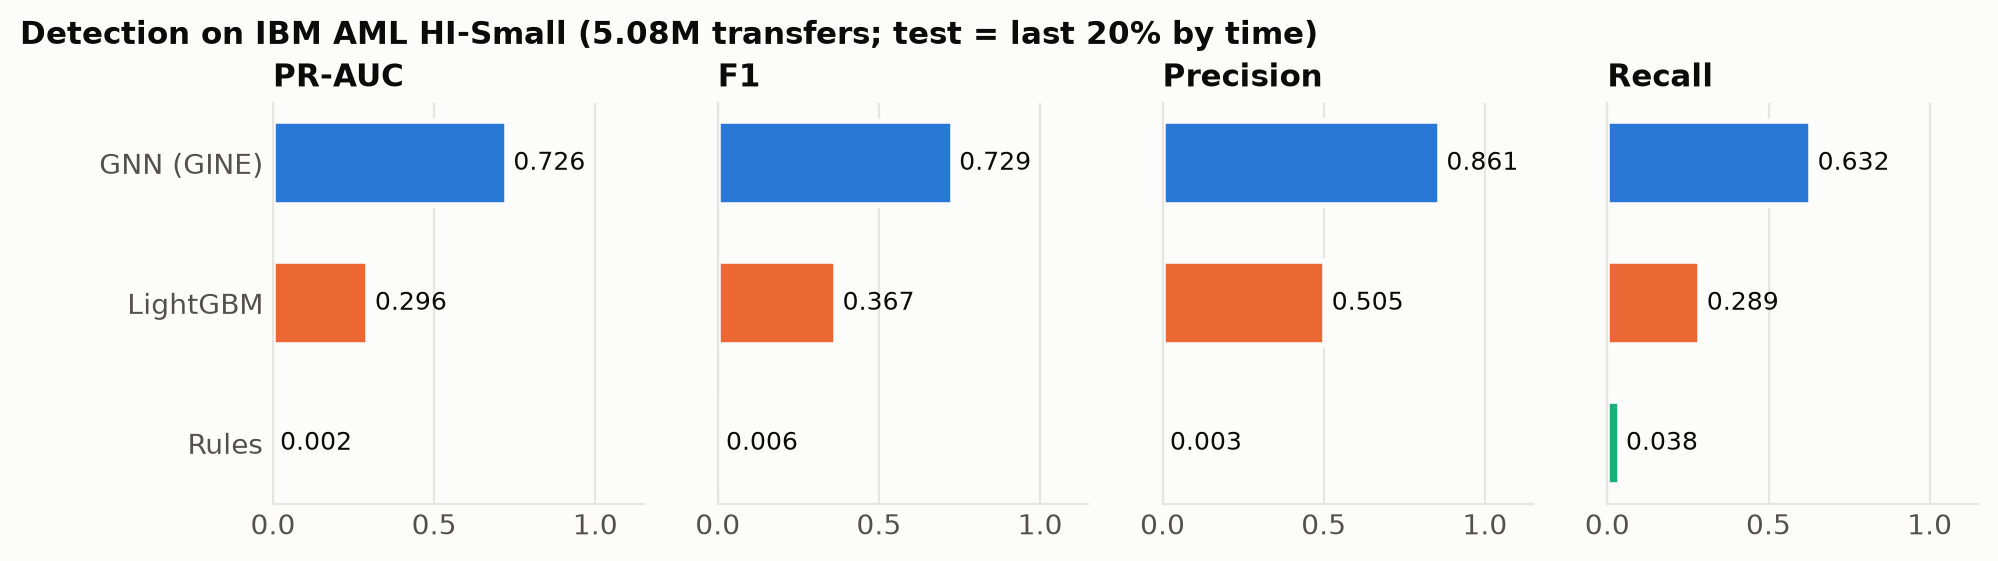
\includegraphics[width=\textwidth]{fig1_hi_small_detection.png}
\caption{Detection metrics on HI-Small (test = last 20\% of transactions by time).}
\label{fig:det}
\end{figure*}

\begin{table}[t]
\caption{Single-operator attacks on the twin: degradation $D$ and recovery $R$ (F1)}
\label{tab:att}
\centering
\setlength{\tabcolsep}{3.2pt}
\begin{tabular}{lcccc}
\toprule
 & \multicolumn{2}{c}{LightGBM} & \multicolumn{2}{c}{GNN} \\
\cmidrule(lr){2-3}\cmidrule(lr){4-5}
Attack & $D$ & $R$ & $D$ & $R$ \\
\midrule
camouflage & +0.481 & +0.330 & +0.436 & +0.313 \\
split & +0.439 & +0.441 & +0.038 & +0.053 \\
mimic & +0.307 & +0.294 & +0.102 & +0.096 \\
delay & +0.011 & +0.002 & +0.000 & $-$0.004 \\
add\_hops & $-$0.005 & +0.019 & $-$0.019 & +0.010 \\
separate\_owners & 0.000 & 0.000 & 0.000 & $-$0.002 \\
\midrule
\textit{clean F1} & \multicolumn{2}{c}{0.974} & \multicolumn{2}{c}{0.971} \\
\bottomrule
\end{tabular}
\end{table}

\begin{figure}[t]
\centering
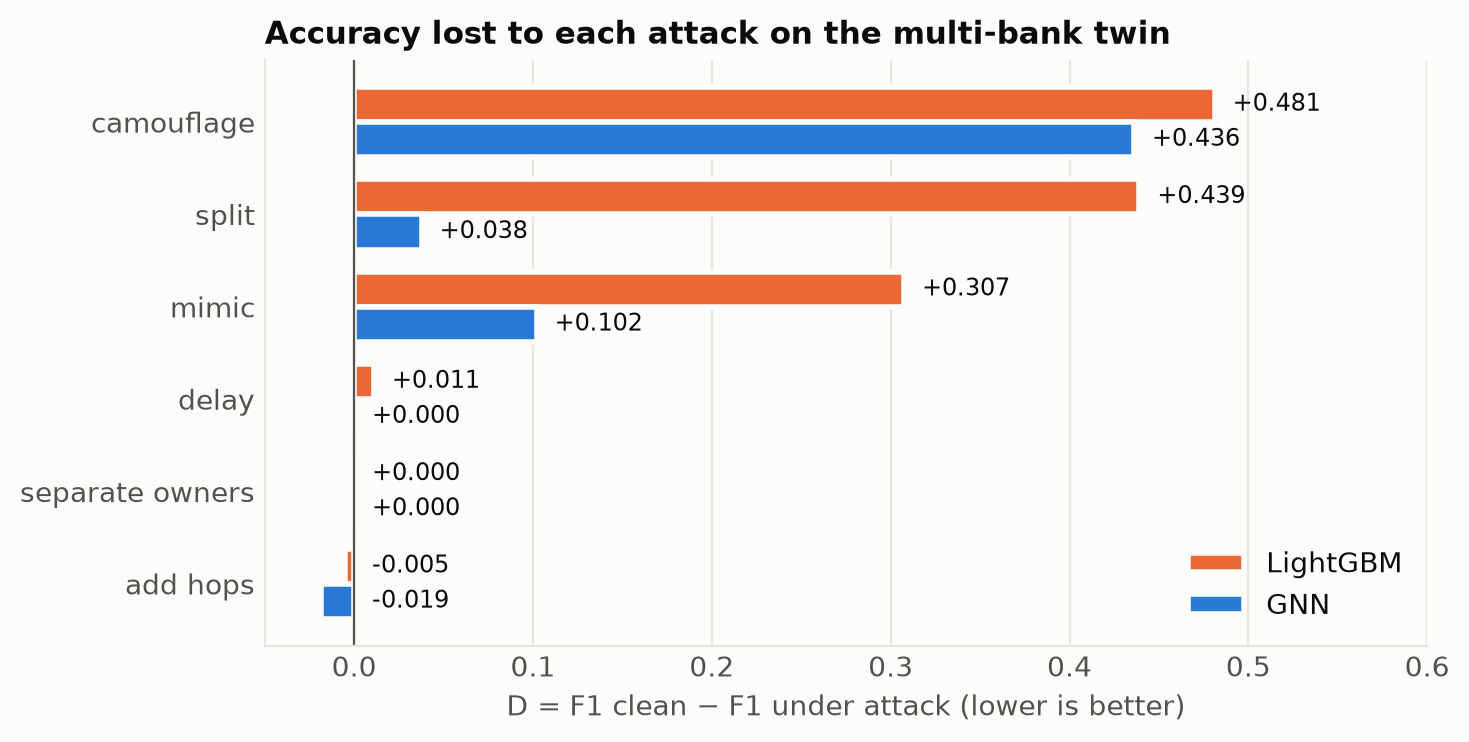
\includegraphics[width=\columnwidth]{fig2_attack_degradation.png}
\caption{Accuracy lost to each attack on the twin ($D$, lower is better).}
\label{fig:att}
\end{figure}

\textbf{Single attacks.} On the clean twin both detectors are strong (F1 0.974 and 0.971). Table~\ref{tab:att} and Fig.~\ref{fig:att} show three regimes. \emph{Structuring} costs LightGBM 0.439 F1 but the GNN only 0.038: split transfers still connect the same accounts, so the graph is unchanged in the ways that matter. \emph{Feature mimicry} --- hiding the observation that 87\% of laundering uses ACH --- costs the GNN a third of what it costs LightGBM. \emph{Relation camouflage} defeats both models ($D$=0.481 and 0.436) and is the only attack that retraining repairs only partly (F1 0.823 and 0.848 after retraining): it attacks neighbourhood aggregation itself, as anticipated by CARE-GNN \cite{dou2020enhancing}. Delays, extra hops and separate owners are absorbed by both detectors.

\begin{figure*}[t]
\centering
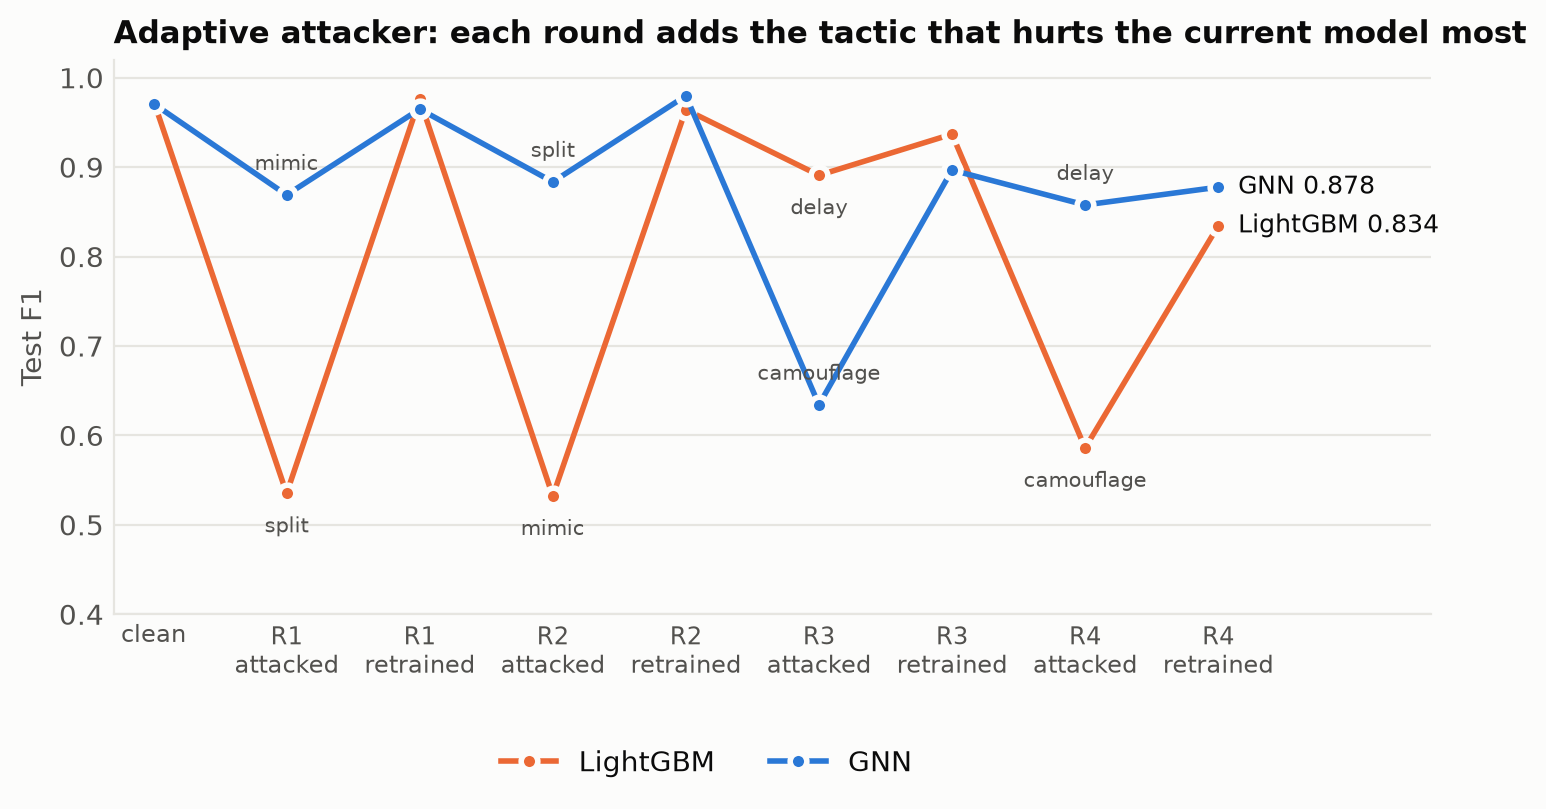
\includegraphics[width=0.82\textwidth]{fig3_adaptive_rounds.png}
\caption{Adaptive attacker. Each round adds the operator that lowers the current detector's validation recall most; points alternate between F1 under attack and after retraining.}
\label{fig:adapt}
\end{figure*}

\textbf{Adaptive attacker.} Fig.~\ref{fig:adapt} shows four rounds. The attacker chose a different first tactic for each model --- structuring against LightGBM and mimicry against the GNN --- i.e.\ it found each model's specific weakness. LightGBM loses 0.44 F1 in each of the first two rounds and the GNN 0.10 and 0.08; both are hurt most when camouflage is added (GNN round 3: 0.980 to 0.634). After four rounds the retrained F1 is 0.878 for the GNN and 0.834 for LightGBM: retraining recovers progressively less as the playbook grows.

\textbf{Investigation agent.} For each of 103 test rings, an investigation opened at the ring's highest-scoring transaction reconstructs the ring by breadth-first search over flagged transactions within $\pm$48 hours, identifies entry and exit accounts, and computes red flags (banks, pass-through time, dormant and shared-owner accounts, fan-in/out, cycles). Against ground truth, reconstruction reaches account precision 0.908, recall 0.989 and Jaccard 0.899, and finds the victim in 95.1\% of rings; under camouflage these fall to 0.743, 0.894, 0.678 and 72.8\%. A language model (gpt-oss-120b \cite{openai2025gptoss}) writes only the report summary through function calls over the case file; every decimal, percentage and stated count is verified against computed facts. In development, the check rejected a draft claiming eight dormant accounts where the case recorded seven.

\section{Discussion and Limitations}
The network view is what makes ring-level detection and robustness to structuring possible, and measuring $D$ and $R$ --- rather than a single accuracy figure --- exposes relation camouflage as the attack AML detectors should be designed against; camouflage-aware aggregation \cite{dou2020enhancing} is a natural next defence. Limitations: twin results are from a single random seed and should be repeated to obtain confidence intervals; all data are synthetic, which is what makes complete ground truth possible but leaves transfer to real bank data open; only the GINE backbone was trained on the full data; and the grounding check verifies numbers and counts, not every qualitative claim.

\section{Conclusion}
ARGUS shows that a heterogeneous, time-respecting GNN detects cross-bank laundering far better than per-transaction models (PR-AUC 0.726 vs.\ 0.296) and is substantially more robust to structuring and feature mimicry, while a controlled digital twin with an adaptive attacker reveals relation camouflage as the open problem. Reporting degradation and recovery alongside accuracy is, we argue, how AML detectors should be evaluated before deployment.

\bibliographystyle{IEEEtran}
\bibliography{refs}

\end{document}
